\begin{figure}
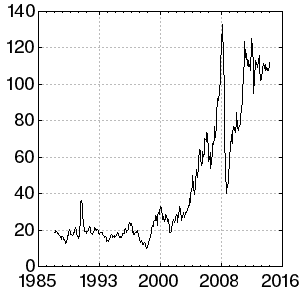
\includegraphics[scale=0.65]{../scripts/oil_gold/oil.png}
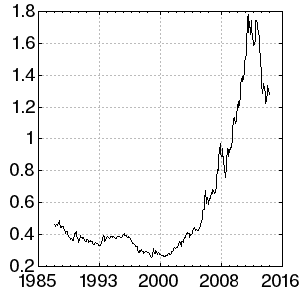
\includegraphics[scale=0.65]{../scripts/oil_gold/gold.png}
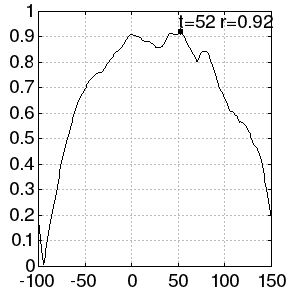
\includegraphics[scale=0.65]{../scripts/oil_gold/result.png}
    \caption{Grafikas kairėje: vidutinė mėnesinė naftos kaina už barelį (USD). Grafikas centre: vidutinė mėnesinė aukso kaina (tūkstančiais USD). Grafikas dešinėje: signalų tarpusavio koreliacija}
\end{figure}

Tirama brent naftos vidutinė mėnesinė kainos\cite{oil} 1987 - 2014 metais koreliacija su aukso mėnesinė vidutine kaina\cite{gold} tuo pačiu laikotarpiu.
Signalų tarpusavio koreliacijos grafikas rodo stiprių ryšį ir turi kelias pagal reikšmę artimas viršūnes.
Didžiausias signalų panašumas yra kai \( R_{fg}(t) = 0.92 \) ir \( t = 52 \).
Bet kitas didelis statistinis panašumas yra kai \( R_{fg}(t) = 0.91 \) ir \( t = 0 \).

